\documentclass{article}
\PassOptionsToPackage{numbers,sort&compress}{natbib}
\usepackage[preprint]{neurips_2026}
\usepackage[utf8]{inputenc}
\usepackage[T1]{fontenc}
\usepackage{hyperref}
\hypersetup{hidelinks}
\usepackage{url}
\usepackage{booktabs}
\usepackage{amsfonts}
\usepackage{amsmath}
\usepackage{microtype}
\usepackage{graphicx}
\usepackage{xcolor}
\usepackage{needspace}
\newcommand{\doi}[1]{\href{https://doi.org/#1}{doi:\,#1}}
\setlength{\textfloatsep}{7pt}
\setlength{\floatsep}{5pt}
\setlength{\intextsep}{5pt}
\setlength{\abovecaptionskip}{3pt}
\setlength{\belowcaptionskip}{0pt}
\setlength{\emergencystretch}{2em}
\setlength{\tabcolsep}{3pt}

\makeatletter
\renewcommand{\@noticestring}{ES 678 Course Project}
\makeatother

\title{Beyond Genres: Finding Your Next Favourite Movie}

\author{%
  \textbf{Rakesh Kumar R} \\
  Roll Number: 26210174 \\
  ES 678 \\
  Indian Institute of Technology Gandhinagar
}

\makeatletter
\renewcommand{\maketitle}{%
  \twocolumn[\@maketitle]%
  \thispagestyle{empty}%
  \@notice
  \let\maketitle\relax
  \let\thanks\relax
}
\makeatother

\renewenvironment{abstract}%
{%
  \vskip 0.075in%
  \begin{center}%
  \begin{minipage}{0.96\columnwidth}%
  \centering
  {\large\bfseries Abstract\par}%
  \vspace{0.5ex}%
  \itshape
}
{%
  \par\end{minipage}%
  \end{center}%
  \vskip 1ex%
}

\begin{document}
\maketitle

\begin{abstract}
On full-catalogue top-10 ranking, a most-popular baseline is difficult to
beat (Table~\ref{tab:val}): its test NDCG@10 is 0.04362 chronologically and
0.08235 under random per-user splitting, compared with 0.03955 and 0.06812
for validation-RMSE-selected MF B. NDCG-selected MF B reaches 0.04354 and
0.07635, but does not exceed popularity. NDCG selection improves both MF A
and MF B with bootstrap CIs excluding zero. On the random split, validation
selects z-score fusion at $\alpha=0.8$; the resulting test hybrid reaches
0.08120, below popularity (Table~\ref{tab:split_sensitivity}). These results
are specific to the
implementations, splits, and one training seed; they are not a claim about
real-world recommendation quality.
\end{abstract}

\section{Question and Setting}
We ask whether a simple popularity ranker is difficult to beat by learned
models, and whether selecting matrix factorization (MF) by validation RMSE
versus validation NDCG changes ranking outcomes. Supporting analyses compare
the two regularization formulations, assess protocol sensitivity, and test
validation-selected score fusion. These implementation-specific comparisons do not show that latent factors
generally dominate content models. Rating prediction and top-$N$ ranking
assess different objectives~\cite{cremonesi2010}; relevance is a held-out
rating $\geq4$, not user satisfaction.

\section{Data and Preparation}
MovieLens 1M \cite{harper2015} contains 1,000,209 ratings (integer 1--5)
from 6,040 users on 3,883 movies, timestamped 2000--2003.
There are no missing values or duplicate user--movie interactions; the
matrix is 95.74\% sparse, median user history is 96, and 57.5\% of ratings
are 4 or 5. Among the 3,706 movies with at least one rating, exposure is
long-tailed (median 123.5 ratings; range 1--3,428); the catalogue contains
177 additional movies with no ratings. Demographics were not used.

The locked per-user chronological split orders each user's ratings by
timestamp (source row order breaks ties) and assigns whole timestamp groups
to the nearest cumulative 80\% and 90\% boundaries. No timestamp tie crosses
partitions. Train, validation, and test contain 799,076, 100,613, and
100,520 ratings. This per-user chronological split preserves each user's
interaction order, but it is not a global timepoint split: training can
include interactions later than held-out interactions from other users. It
therefore provides a more temporally ordered within-user evaluation than
random splitting, but does not reproduce a strict system-wide deployment
cutoff. The training mean is $\mu=3.6170$. The separate random per-user
split (80/10/10, seed 42) has 797,758/97,383/105,068
train/validation/test rows and a training mean of 3.5805; it ignores
timestamp order and evaluates held-out interactions, not future
recommendations.

\section{Models}
\paragraph{Bias and popularity baselines.}
The regularized baseline predicts $\hat r_{ui}=\mu+b_u+b_i$ from training
ratings, capturing user and item biases but no interaction. It uses user/movie
regularization 5 and 15 iterations. Because $b_u$ is constant within a user's
list, its ranking depends on item bias. The separate most-popular baseline
ranks movies by their training interaction count.

\paragraph{Biased matrix factorization.}
Following the standard latent-factor formulation, MF predicts
\begin{equation}
  \begin{aligned}
  \hat r_{ui}&=\mu+b_u+b_i+\mathbf p_u^\top\mathbf q_i,\\
  e_{ui}&=r_{ui}-\hat r_{ui}.
  \end{aligned}
\end{equation}
Both compared formulations use mini-batch summed squared error and $L_2$
regularization. For batch $\mathcal B$, let $n_u$ and $n_i$ count
interactions involving user $u$ and movie $i$, respectively. Formulation A
counts an entity's penalty once per interaction; B counts each distinct
entity once:
\begin{equation}
  \begin{aligned}
  J_A(\mathcal B)&=\frac12\sum_{(u,i)\in\mathcal B}e_{ui}^2\\
  &\quad+\frac{\lambda}{2}\sum_{(u,i)\in\mathcal B}
       (b_u^2+\|\mathbf p_u\|_2^2)\\
  &\quad+\frac{\lambda}{2}\sum_{(u,i)\in\mathcal B}
       (b_i^2+\|\mathbf q_i\|_2^2).
  \end{aligned}
\end{equation}
\begin{equation}
  \begin{aligned}
  J_B(\mathcal B)&=\frac12\sum_{(u,i)\in\mathcal B}e_{ui}^2\\
  &\quad+\frac{\lambda}{2}\sum_{u\in U_{\mathcal B}}
       (b_u^2+\|\mathbf p_u\|_2^2)\\
  &\quad+\frac{\lambda}{2}\sum_{i\in I_{\mathcal B}}
       (b_i^2+\|\mathbf q_i\|_2^2).
  \end{aligned}
\end{equation}
For a user with $n_u$ occurrences in a batch, the factor gradient and update
are
\[
\begin{aligned}
 \nabla_{p_u}J_A
   &=-\sum_{i\in B_u}e_{ui}q_i+\lambda n_up_u,\\
 p_u^+
   &=p_u+\eta\{\sum_{i\in B_u}e_{ui}q_i-\lambda n_up_u\},\\
 \nabla_{p_u}J_B
   &=-\sum_{i\in B_u}e_{ui}q_i+\lambda p_u,\\
 p_u^+
   &=p_u+\eta\{\sum_{i\in B_u}e_{ui}q_i-\lambda p_u\}.
\end{aligned}
\]
The same expressions hold for biases and movie parameters. Thus A's
shrinkage is $\eta\lambda n_u$ per update, while B's is $\eta\lambda$;
popular entities are over-regularized by A for a fixed batch size.

\begin{table}[!ht]
\centering
\caption{Matched-$\lambda$ validation comparison on the per-user
chronological split. Factors and epoch were selected by validation RMSE; NDCG
is reported on that partition.}
\label{tab:matched}
\scriptsize
\setlength{\tabcolsep}{3pt}
\begin{tabular}{crrrr}
\toprule
$\lambda$ & A factors & A RMSE/NDCG & B factors & B RMSE/NDCG\\
\midrule
.02 & 10 & .87324/.02722 & 10 & .87856/.03589\\
.05 & 50 & .86547/.02928 & 10 & .87275/.03733\\
.10 & 50 & .88064/.01281 & 10 & .86738/.04136\\
\bottomrule
\end{tabular}
\end{table}
Across matched lambdas, A wins validation RMSE at .02 and .05, while B wins
at .10; B wins validation NDCG for all three. Search uses 10/20/50 factors, $\lambda\in\{.02,.05,.1\}$, learning rate .01,
batch size 8,192, and seed 42. Clipping is used only for RMSE/MAE; primary
ranking uses unclipped MF scores. For corrected MF B, clipped test rankings
contained 37,094/13,016 tied candidates/top-10 slots chronologically and
32,640/13,237 randomly; unclipped NDCG@10 was 0.03955/0.06812 versus
0.03959/0.06793 clipped.
At $\lambda=.10$, A's validation NDCG drops to 0.01281 while B reaches
0.04136, consistent with A's shrinkage scaling as $\lambda n_u$.

\paragraph{Genre content.}
Each movie has a binary multi-hot genre vector $\mathbf x_i$. From training
ratings only, user $u$'s profile and movie score are
\begin{equation}
 \begin{aligned}
 \mathbf g_u&=\mathrm{L2Norm}(\sum_{j\in I_u^{\rm train}}
       (r_{uj}-\mu)\mathbf x_j),\\
 s_{\rm genre}(u,i)&=\frac{\mathbf g_u^\top\mathbf x_i}{\|\mathbf x_i\|_2}.
 \end{aligned}
\end{equation}
Mean-centering lets ratings above/below the mean increase/decrease genre
directions. Cosine scores lie in $[-1,1]$; zero profiles or unknown IDs score
zero. Ties use ascending movie ID; no user had a zero profile.

\section{Evaluation Protocol}
Candidates are the full catalogue minus each user's training-rated movies,
identical within a comparison. Validation selects models and fusion weights;
each frozen configuration, including hybrids, is evaluated once on test. Of
the two protocols, per-user chronological
evaluation better preserves within-user order for future-interaction
prediction than random per-user splitting. It is not a global timepoint
split: training may include later interactions than another user's held-out
interaction, so it does not simulate a system-wide deployment cutoff.
Random per-user splitting is a held-out-interaction
evaluation, not a future-time evaluation. Candidate choice and user
eligibility also affect offline metrics. Both splits use
relevance rating $\geq4$; $H_u$ counts relevant top-10 movies and $R_u$ is
the set of distinct relevant held-out movies. We report
Precision@10 $=H_u/10$, Recall@10 $=H_u/|R_u|$, and binary-gain
NDCG@10 $=\mathrm{DCG}_u/\mathrm{IDCG}_u$, where
$\mathrm{DCG}_u=\sum_{r=1}^{10}y_{ur}/\log_2(r+1)$ and ideal DCG sums the
first $\min(10,|R_u|)$ gains; $y_{ur}$ is binary relevance at rank $r$.
Metrics are macro-averaged. Zero-relevant users remain in Precision and are
excluded from Recall/NDCG (263 of the 6,039 users with validation
interactions; 272 of 6,040 test users). One user has no validation interactions in the per-user chronological split
and is therefore absent from validation ranking.
Unrated candidates are unjudged, not confirmed negatives; we make no
cross-paper performance claim.

\section{Results}
\begin{table*}[t]
\centering
\caption{Full-catalogue Precision@10, Recall@10, and NDCG@10 for the
per-user chronological split.}
\label{tab:val}
\small
\begin{tabular}{lrrrrrr}
\toprule
& \multicolumn{3}{c}{Validation} & \multicolumn{3}{c}{Test}\\
Model & P@10 & Recall@10 & NDCG@10 & P@10 & Recall@10 & NDCG@10\\
\midrule
Bias baseline & 0.01563 & 0.01701 & 0.01683 & 0.01417 & 0.01628 & 0.01587\\
Most popular & 0.03355 & \textbf{0.04187} & \textbf{0.04824} & 0.02975 & \textbf{0.04026} & \textbf{0.04362}\\
MF A (RMSE) & 0.02191 & 0.02647 & 0.02940 & 0.02075 & 0.02674 & 0.02833\\
MF B (RMSE) & 0.02986 & 0.03546 & 0.04187
& 0.02775 & 0.03446 & 0.03955\\
MF A (NDCG; post-hoc) & 0.02653 & 0.02953 & 0.03496 & 0.02485 & 0.02796 & 0.03307\\
MF B (NDCG; post-hoc) & 0.03348 & 0.03814 & 0.04652 & 0.03073 & 0.03746 & 0.04354\\
Genre & 0.00758 & 0.01213 & 0.01145 & 0.00586 & 0.00988 & 0.00852\\
\bottomrule
\end{tabular}
\end{table*}

Table~\ref{tab:val} shows that popularity has the highest Recall@10 and
NDCG@10, while MF B has the highest P@10 among the learned models. The
full-grid RMSE-selected MF B has validation/test RMSE 0.86738/0.88638; the
matched lambda=.10 row is therefore its selected configuration. Selecting by
validation NDCG changes its configuration and raises test NDCG from 0.03955
to 0.04354. The NDCG-selected variants are post-hoc analyses
added after the first standalone test results were already seen, not new
test-blind model selections.
For both rules the grid is 10/20/50 factors and
$\lambda\in\{.02,.05,.10\}$, with learning rate .01, batch size 8,192,
seed 42, and early stopping after four non-improving validation checkpoints.
The retained (factors, $\lambda$, epoch) configurations are, respectively,
chronological RMSE: A (50,.05,22), B (10,.10,29); chronological NDCG:
A (50,.02,11), B (20,.10,20); random RMSE: A (50,.05,24), B (10,.10,30);
and random NDCG: A (20,.02,14), B (20,.10,17).

\paragraph{Random per-user sensitivity.}
We shuffled rating rows within users (seed 42) and assigned 80/10/10.
Table~\ref{tab:split_sensitivity} compares the protocols. Random splitting
evaluates held-out interactions rather than future-time recommendations, so
its higher scores are not evidence of better recommendation quality.
\begin{table*}[t]
\centering
\caption{Full-catalogue NDCG@10 under per-user chronological and random
per-user evaluation. Test change is the relative difference between
protocols, not a model improvement.}
\label{tab:split_sensitivity}
\small
\begin{tabular}{lrrrrr}
\toprule
& \multicolumn{2}{c}{Validation} & \multicolumn{2}{c}{Test} & Test change\\
Model & \shortstack{Per-user\\chronological} & \shortstack{Random\\per-user}
& \shortstack{Per-user\\chronological} & \shortstack{Random\\per-user}
& \shortstack{Random vs.\\per-user chronological}\\
\midrule
Bias & 0.01683 & 0.02595 & 0.01587 & 0.02653 & +67.2\%\\
Most popular & 0.04824 & 0.08174 & \textbf{0.04362} & \textbf{0.08235} & +88.8\%\\
MF A (RMSE) & 0.02940 & 0.04955 & 0.02833 & 0.05089 &  +79.7\%\\
MF B (RMSE) & 0.04187 & 0.06693 & 0.03955 & 0.06812 & +72.2\%\\
MF A (NDCG; post-hoc) & 0.03496 & 0.05363 & 0.03307 & 0.05471 & +65.5\%\\
MF B (NDCG; post-hoc) & 0.04652 & 0.07662 & 0.04354 & 0.07635 & +75.4\%\\
Genre & 0.01145 & 0.01292 & 0.00852 & 0.01446 & +69.7\%\\
\bottomrule
\end{tabular}
\end{table*}
The protocols measure different held-out populations; random scores are not
future-time performance estimates.

\paragraph{History-length and failure analysis.}
On the random per-user split, validation NDCG@10 by training-history group is
shown in Table~\ref{tab:history}; the corresponding protocol curves are in
Figure~\ref{fig:protocol}.
\begin{table}[!ht]
\centering
\caption{Random per-user validation NDCG@10 by training-history length.}
\label{tab:history}
\small
\begin{tabular}{lrrrr}
\toprule
History & Users & MF B & Popular & Genre\\
\midrule
6--20 & 553 & 0.02342 & 0.06640 & 0.01194\\
21--50 & 1,674 & 0.03888 & 0.05925 & 0.01080\\
51+ & 3,813 & 0.08384 & 0.09294 & 0.01392\\
\bottomrule
\end{tabular}
\end{table}
MF B is below popularity in all three groups; the gap is largest for 6--20
and 21--50 histories and nearly closes at 51+. This descriptive pattern is
consistent with latent factors being harder to estimate from short histories.
Genre changes little, and genre tags omit within-genre distinctions, actors,
and sequencing.

\section{Does Score Fusion Help?}
MF scores are unclipped predictions for ranking and are clipped to $[1,5]$
only for rating error; Genre scores are cosine values in
$[-1,1]$, so raw addition is not justified. Weighted fusion is a standardized hybrid strategy. For each user, scores are
standardized across eligible candidates,
$z_{um}=(s_{um}-\bar{s}_u)/\max(\sigma_u,10^{-8})$, then combined as
$\alpha z^{\rm MF}_{um}+(1-\alpha)z^{\rm genre}_{um}$ for
$\alpha=0,0.1,\ldots,1$. The population-standard-deviation floor prevents
division by zero; endpoints reproduce standalone rankings. The original
rank-fusion comparator maps descending rank position $j$ among $n$
candidates to $1-j/(n-1)$ before weighted addition.

\begin{figure*}[t]
\centering
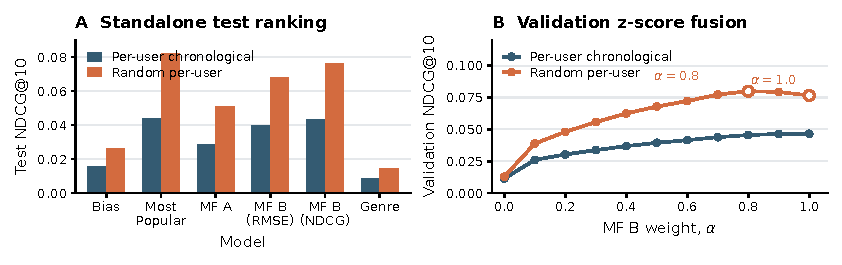
\includegraphics[width=\textwidth]{split_fusion_history.pdf}
\caption{(A) Standalone test NDCG@10 under per-user chronological and random
per-user evaluation, including the full-grid validation-RMSE MF B and
post-hoc NDCG-selected MF B. (B) Validation z-score fusion curves using
NDCG-selected MF B;
markers identify the selected random per-user $\alpha=0.8$ and chronological
$\alpha=1.0$ values.}
\label{fig:protocol}
\end{figure*}

The curves use NDCG-selected MF B: chronological validation selected
$\alpha=1$ (NDCG@10 0.04652), while random validation selected $\alpha=0.8$
(0.07999 versus 0.07662 for its standalone base). The corresponding test
hybrid reached 0.08120, below popularity at 0.08235 (Table~\ref{tab:split_sensitivity}).
Fusion performance is protocol-dependent and
does not establish general hybrid superiority. Per-user chronological MF B/Genre lists had mean overlap
0.053 movies (0.0053 of the 10-item list), mean Jaccard 0.0028, and
candidate-wise Spearman correlation 0.130. Low overlap or rank similarity
alone does not establish relevance complementarity. These fusion results are
validation-selected. Paired user bootstrap intervals (1,000 resamples, seed
42) include Popular$-$MF B (NDCG) [-0.00290,0.00328] chronologically and
Popular$-$hybrid [-0.00303,0.00506] randomly, so those differences are
indistinguishable; NDCG$-$RMSE intervals exclude zero for both MF A
[0.00328,0.00626] chronologically and [0.00157,0.00621] randomly, and MF B
[0.00185,0.00601] and [0.00560,0.01102]. They do not resample training
seeds; all models use one seed.

\section{Limitations and Conclusion}
MovieLens 1M is an older, single-domain benchmark. The per-user chronological
split is static and does not reproduce a global deployment cutoff; unrated
candidates are unjudged.
MF has no learned factors for unseen users or movies, whereas genre metadata
can score a movie for a user with a nonzero profile; cold-start performance
was not measured. Popularity is the strongest simple baseline in these full-catalogue tests:
it is statistically indistinguishable from both MF B variants chronologically
and exceeds both under random splitting. Its advantage over the random hybrid
is uncertain under the paired bootstrap. NDCG selection improves both MF A and
MF B ranking with CIs excluding zero; MF B remains clearly above MF A. The
random split gives higher scores for a
different, non-future task. The regularization comparison is not causal; no
repeated temporal splits or batch-size sensitivity tests were run. These
results are limited to MovieLens 1M, these implementations, these protocols,
and one training seed; validation on other domains and preferably online or
user-centred evaluation is needed before generalising.

\section{Reproducibility and AI-Use Disclosure}
Code, setup, MovieLens 1M download, and reproduction commands are in the
README at \url{https://github.com/rakesh91/movieRec}. An AI assistant using
Copilot SDK in VS Code assisted with coding, reproducibility checks,
documentation wording, and formatting. The research question, analysis,
interpretation, experimental design decisions, and ideation were by the
author, who ran and verified the experiments and remains responsible for the
code, results, paper, and conclusions.

\tiny
\begin{thebibliography}{9}
\bibitem[Cremonesi et~al.(2010)]{cremonesi2010}
P. Cremonesi, Y. Koren, and R. Turrin.
\newblock Performance of Recommender Algorithms on Top-N Recommendation
Tasks.
\newblock In \emph{RecSys '10}, pages 39--46, 2010.

\bibitem[Harper and Konstan(2015)]{harper2015}
F. M. Harper and J. A. Konstan.
\newblock The MovieLens Datasets: History and Context.
\newblock \emph{ACM Transactions on Interactive Intelligent Systems},
5(4):19:1--19:19, 2015.

\end{thebibliography}

\end{document}
